% !TEX root = ../tex/5-2.tex
% 第5章：本文は青、補足は緑
\newcommand{\asmain}{%
    \setbeamercolor{frametitle}{fg=white,bg=main}%
    \setbeamercolor{structure}{fg=main}%
    \setbeamercolor{itemize item}{fg=main}%
    \setbeamercolor{itemize subitem}{fg=main}%
    \setbeamercolor{enumerate item}{fg=main}%
}
\newcommand{\assuppl}{%
    \setbeamercolor{frametitle}{fg=white,bg=examplecol}%
    \setbeamercolor{structure}{fg=examplecol}%
    \setbeamercolor{itemize item}{fg=examplecol}%
    \setbeamercolor{itemize subitem}{fg=examplecol}%
    \setbeamercolor{enumerate item}{fg=examplecol}%
}
% フレームタイトルの「補足」だけを□で囲む
\newcommand{\supplmark}{%
    \setlength{\fboxsep}{1.5pt}%
    \setlength{\fboxrule}{0.7pt}%
    \fbox{\textbf{補足}}%
}
\asmain


%=============================================
\begin{frame}{5.1から5.2へ}
    \begin{block}{ここまで（5.1）}
        NFの可逆写像と、NODEの連続速度場。\\
        尤度学習はODEソルバを繰り返し呼ぶ必要があり重い。
    \end{block}
    \begin{block}{ここから（5.2）}
        Flow Matching：速度場を回帰で直接学ぶ。\\
        条件付き速度の平均が周辺速度になる、というDSM型の原理。
    \end{block}
\end{frame}
%=============================================
\asmain
\begin{frame}{5.2 の位置づけ}
    \begin{block}{この節の役割}
        「スコア経由」ではなく「速度を直接」学ぶ枠組みを定式化する
    \end{block}
    \begin{enumerate}
        \item \textbf{5.2.1 スコア法からの教訓}\\
        条件付き$\to$周辺、および速度への読み替え
        \item \textbf{5.2.2 Flow Matching}\\
        $p_{\mathrm{src}}\to p_{\mathrm{tgt}}$、CFM目的関数（5.2.10）
        \item \textbf{5.2.3 比較}\\
        Diffusion／一般FM／NODE
        \item \textbf{5.2.4（任意）}\\
        連続の方程式と周辺速度の正当性
    \end{enumerate}
\end{frame}
%=============================================
\section{スコア法からの教訓}
\asmain
\begin{frame}{区切り：スコア法からの教訓}
    \tableofcontents[currentsection]
\end{frame}
%=============================================
\asmain
\begin{frame}{NODEの限界とFMの狙い}
    Score SDEもNODEも、連続輸送で$p_{\mathrm{prior}}\leftrightarrow p_{\mathrm{data}}$を考える。
    \begin{itemize}
        \item NODE：確定的ODEを直接パラメータ化し、最尤で学ぶ\\
        $\Rightarrow$学習中にODEを解く（高い）
        \item Flow Matching：速度を回帰で予測（v-prediction）\\
        $\Rightarrow$学習はシミュレーションフリー、生成時だけ積分
    \end{itemize}
    \begin{block}{一般化}
        端点はガウス$\to$データに限らない。\\
        $p_{\mathrm{src}}$と$p_{\mathrm{tgt}}$（どちらもサンプル可能）の間の輸送。
    \end{block}
\end{frame}
%=============================================
\asmain
\begin{frame}{図5.6：条件付き遷移分布}
    \centering
    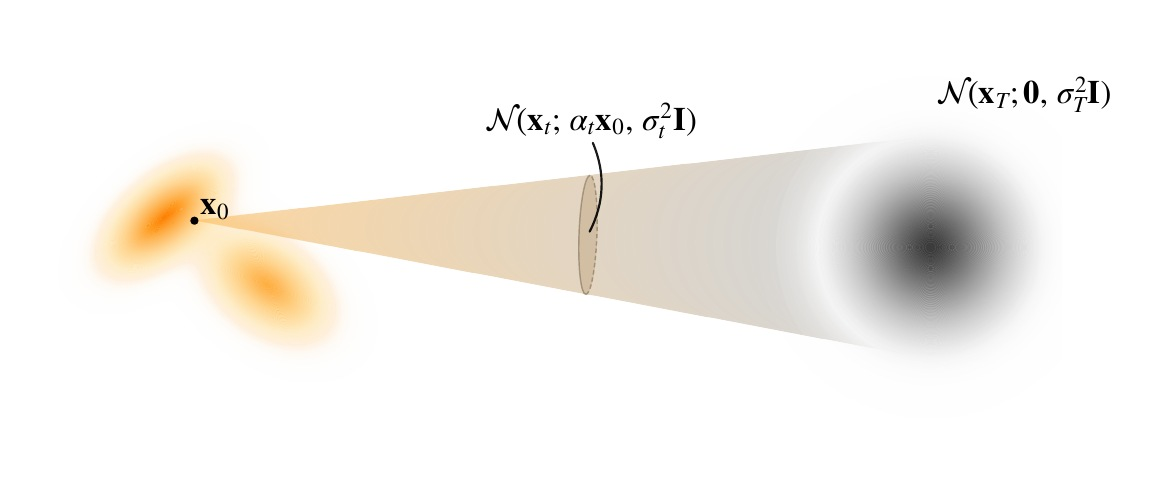
\includegraphics[width=\textwidth,height=0.58\textheight,keepaspectratio]{fig-5-6.jpg}
    \vfill
    \footnotesize
    $p_t(\bm{x}_t|\bm{x}_0)=\mathcal{N}(\bm{x}_t;\alpha_t\bm{x}_0,\sigma_t^{2}\bm{I})$（式5.2.1）。\\
    固定データ$\bm{x}_0$からガウス事前へ広がる条件付き経路。
\end{frame}
%=============================================
\asmain
\begin{frame}{条件付き経路と周辺}
    拡散モデルの時間家族（ここでは$t=0$がデータ、$t=1$が事前）：
    \[
        p_t(\bm{x}_t|\bm{x}_0)
        =
        \mathcal{N}(\bm{x}_t;\alpha_t\bm{x}_0,\sigma_t^{2}\bm{I}),
        \qquad
        \bm{x}_0\sim p_{\mathrm{data}}
        \tag{5.2.1}
    \]
    周辺は
    \[
        p_t(\bm{x}_t)
        =
        \int p_t(\bm{x}_t|\bm{x}_0)\,p_{\mathrm{data}}(\bm{x}_0)\,d\bm{x}_0
    \]
    \begin{block}{要点}
        条件付きは閉じた形。周辺$p_t$自体は一般に扱いにくい。
    \end{block}
\end{frame}
%=============================================
\asmain
\begin{frame}{PF-ODE速度とスコア}
    Fokker--Planckから決まる決定的速度：
    \[
        \bm{v}_t(\bm{x})
        :=
        f(t)\bm{x}
        -
        \tfrac12 g^{2}(t)\,\nabla_{\bm{x}}\log p_t(\bm{x})
        \tag{5.2.2}
    \]
    対応するPF-ODEは$\dot{\bm{x}}(t)=\bm{v}_t(\bm{x}(t))$。
    \begin{itemize}
        \item スコアを学べば速度が組み立てられる（第4章）
        \item 周辺スコアは未知$\Rightarrow$条件付きスコアへ回帰（DSM）
    \end{itemize}
\end{frame}
%=============================================
\asmain
\begin{frame}{条件付きから周辺へ（スコア）}
    \[
        \nabla_{\bm{x}_t}\log p_t(\bm{x}_t)
        =
        \mathbb{E}_{\bm{x}_0\sim p(\cdot|\bm{x}_t)}
        \bigl[
        \nabla_{\bm{x}_t}\log p_t(\bm{x}_t|\bm{x}_0)
        \bigr]
        \tag{5.2.3}
    \]
    同じ原理を速度に移すと、条件付き速度
    \[
        \bm{v}_t(\bm{x}_t|\bm{x}_0)
        :=
        f(t)\bm{x}_t
        -
        \tfrac12 g^{2}(t)\,\nabla_{\bm{x}_t}\log p_t(\bm{x}_t|\bm{x}_0)
    \]
    について
    \[
        \bm{v}_t(\bm{x}_t)
        =
        \mathbb{E}_{\bm{x}_0\sim p(\cdot|\bm{x}_t)}
        \bigl[\bm{v}_t(\bm{x}_t|\bm{x}_0)\bigr]
    \]
\end{frame}
%=============================================
\asmain
\begin{frame}{図5.7：条件付き視点と周辺視点}
    \centering
    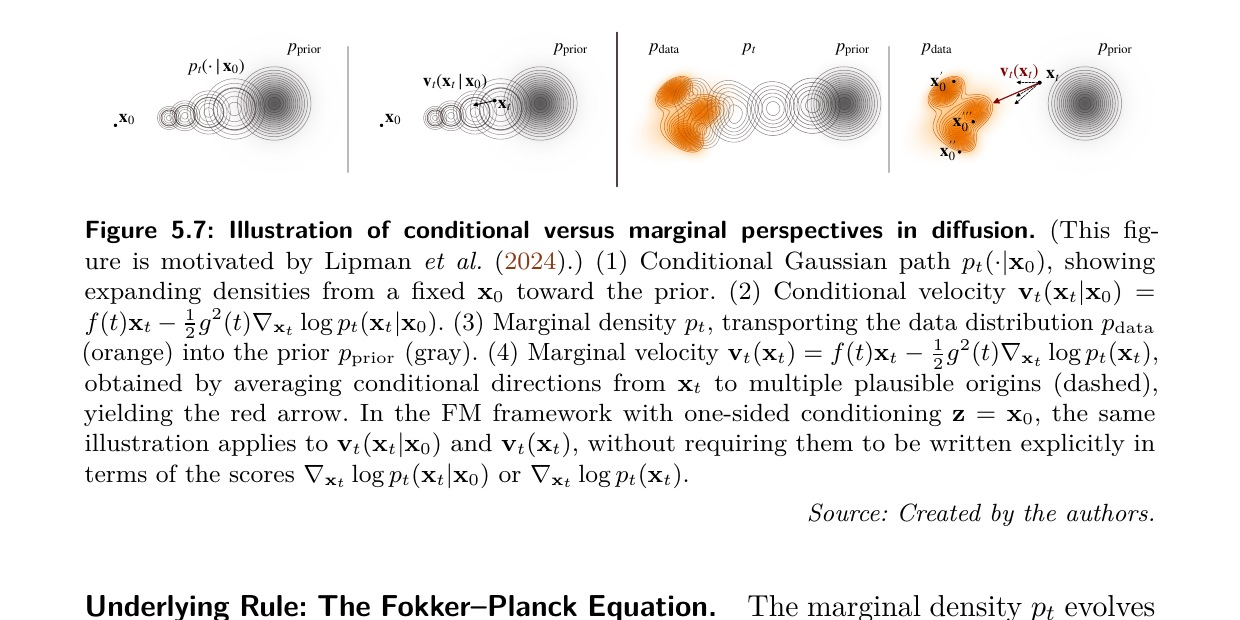
\includegraphics[width=\textwidth,height=0.58\textheight,keepaspectratio]{fig-5-7.jpg}
    \vfill
    \footnotesize
    (1)(2) 条件付き密度／速度。\\
    (3)(4) 周辺密度と、複数の起源の平均としての周辺速度（赤矢印）。
\end{frame}
%=============================================
\assuppl
\begin{frame}{\supplmark：図5.7の読み方}
    \begin{enumerate}
        \item 固定$\bm{x}_0$から広がるガウス条件付き経路
        \item その経路上の閉じた条件付き速度（1本の矢印）
        \item データ分布全体が事前へ流れる周辺密度
        \item 点$\bm{x}_t$では複数の$\bm{x}_0$が候補$\Rightarrow$平均が周辺速度
    \end{enumerate}
    \begin{exampleblock}{FMへの含意}
        スコアを経由せずとも、同じ図を$\bm{v}_t(\cdot|\bm{x}_0)$と$\bm{v}_t$で読める。
    \end{exampleblock}
\end{frame}
%=============================================
\asmain
\begin{frame}{教訓のまとめ}
    \begin{itemize}
        \item 拡散は実質「確率流の速度」を学んでいる
        \item 周辺量は難しいが、条件付き量は閉じた教師になる
        \item 同じ条件付け原理を、速度そのものに直接適用できる
    \end{itemize}
    \begin{block}{次}
        一般の$p_{\mathrm{src}}$、$p_{\mathrm{tgt}}$に対するFlow Matchingを定式化する。
    \end{block}
\end{frame}
%=============================================
\section{Flow Matching}
\asmain
\begin{frame}{区切り：Flow Matching}
    \tableofcontents[currentsection]
\end{frame}
%=============================================
\asmain
\begin{frame}{端点と周辺経路}
    任意のソース／ターゲットについて（FMの時刻規約）
    \[
        p_0=p_{\mathrm{src}},
        \qquad
        p_1=p_{\mathrm{tgt}}
        \tag{5.2.6}
    \]
    潜在$z\sim\pi(z)$と条件付き$p_t(\bm{x}_t|z)$で周辺を書く：
    \[
        p_t(\bm{x}_t)
        =
        \int p_t(\bm{x}_t|z)\,\pi(z)\,dz
        \tag{5.2.7}
    \]
    \begin{columns}[T,onlytextwidth]
        \begin{column}{0.48\textwidth}
            \begin{block}{片側条件付け}
                $z=\bm{x}_0$または$\bm{x}_1$。\\
                ガウスソースなら拡散に近い。
            \end{block}
        \end{column}
        \begin{column}{0.48\textwidth}
            \begin{block}{両側条件付け}
                $z=(\bm{x}_0,\bm{x}_1)$。\\
                任意の端点間の輸送向き。
            \end{block}
        \end{column}
    \end{columns}
\end{frame}
%=============================================
\asmain
\begin{frame}{速度場と連続の方程式}
    同じ$\{p_t\}$でも、粒子の動かし方（速度）は一意ではない。\\
    FMの目標：ODE
    \[
        \dfrac{d\bm{x}(t)}{dt}=\bm{v}_t(\bm{x}(t))
    \]
    の周辺が所定の$\{p_t\}$に一致すること。必要条件は
    \[
        \partial_t p_t(\bm{x})
        +
        \nabla\cdot\bigl(\bm{v}_t(\bm{x})\,p_t(\bm{x})\bigr)
        =
        0
        \tag{5.2.8}
    \]
    \begin{block}{注意}
        連続の方程式は密度の進化を縛るが、速度を一意には決めない\\
        （発散ゼロ場を足してもよい）。
    \end{block}
\end{frame}
%=============================================
\asmain
\begin{frame}{理想のFM損失と条件付き構成}
    理想は周辺速度への回帰：
    \[
        \mathcal{L}_{\mathrm{FM}}(\phi)
        =
        \mathbb{E}_{t,\bm{x}_t\sim p_t}
        \bigl\|
        \bm{v}_\phi(\bm{x}_t,t)-\bm{v}_t(\bm{x}_t)
        \bigr\|_{2}^{2}
    \]
    だが$\bm{v}_t$は一般に未知。そこで
    \[
        \bm{v}_t(\bm{x}_t)
        :=
        \mathbb{E}_{z\sim p(\cdot|\bm{x}_t)}
        \bigl[\bm{v}_t(\bm{x}_t|z)\bigr]
        \tag{5.2.9}
    \]
    条件付き速度が経路を正しく運べば、その平均は妥当な周辺速度になる。
\end{frame}
%=============================================
\asmain
\begin{frame}{条件付きFlow Matching（CFM）}
    \[
        \resizebox{0.98\textwidth}{!}{$
        \mathcal{L}_{\mathrm{CFM}}(\phi)
        :=
        \mathbb{E}_{t,\,z\sim\pi,\,\bm{x}_t\sim p_t(\cdot|z)}
        \bigl\|
        \bm{v}_\phi(\bm{x}_t,t)-\bm{v}_t(\bm{x}_t|z)
        \bigr\|_{2}^{2}
        $}
        \tag{5.2.10}
    \]
    \begin{itemize}
        \item $z$は教師$\bm{v}_t(\bm{x}_t|z)$とサンプル$\bm{x}_t$を作るためだけに使う\\
        （ネット入力は$(\bm{x}_t,t)$）
        \item $\mathcal{L}_{\mathrm{FM}}=\mathcal{L}_{\mathrm{CFM}}+C$（$C$は$\phi$に独立）
        \item 最小化子は周辺速度$\bm{v}^{\star}(\bm{x}_t,t)=\bm{v}_t(\bm{x}_t)$（式5.2.11）
    \end{itemize}
\end{frame}
%=============================================
\asmain
\begin{frame}{図5.8：FMにおける条件付けトリック}
    \centering
    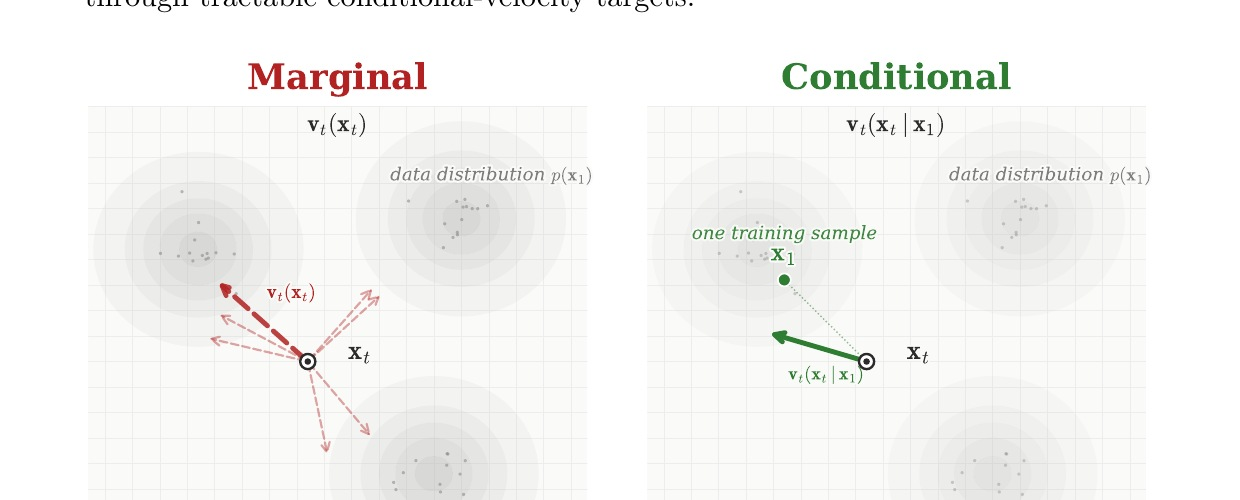
\includegraphics[width=\textwidth,height=0.58\textheight,keepaspectratio]{fig-5-8.jpg}
    \vfill
    \footnotesize
    左：周辺速度は全ターゲットの寄与の平均（扱いにくい）。\\
    右：訓練時は既知の$\bm{x}_1$に対する閉じた条件付き速度を回帰する。
\end{frame}
%=============================================
\assuppl
\begin{frame}{\supplmark：定理5.2.1（LFMとLCFMの同値）}
    \[
        \mathcal{L}_{\mathrm{FM}}(\phi)
        =
        \mathcal{L}_{\mathrm{CFM}}(\phi)+C
    \]
    共通の最小化子は、ほとんどすべての$\bm{x}_t\sim p_t$で
    \[
        \bm{v}^{\star}(\bm{x}_t,t)=\bm{v}_t(\bm{x}_t)
    \]
    （定義は式5.2.9）。
    \begin{exampleblock}{位置づけ}
        変分（定理2.2.1）・DSM（定理3.3.1）に続く、\\
        条件付けトリックの第3の現れ（図5.8）。
    \end{exampleblock}
\end{frame}
%=============================================
\asmain
\begin{frame}{シミュレーションフリーのための条件}
    CFMが実用になるには：
    \begin{enumerate}
        \item[(i)] $\bm{x}_t\sim p_t(\cdot|z)$がODEなしでサンプルできる
        \item[(ii)] 教師$\bm{v}_t(\bm{x}_t|z)$が閉じた形（または安い式）で書ける
    \end{enumerate}
    \begin{block}{次節への予告}
        具体的な条件付き経路・速度の作り方は5.3（確率経路の構成）。
    \end{block}
\end{frame}
%=============================================
\asmain
\begin{frame}{FM本体のまとめ}
    \begin{itemize}
        \item 所定の$\{p_t\}$を実現する速度を、ネット$\bm{v}_\phi$で直接学ぶ
        \item 周辺速度は条件付き速度の平均（5.2.9）
        \item CFM（5.2.10）はDSMと同じく、条件付き教師で周辺を回復する
    \end{itemize}
\end{frame}
%=============================================
\section{比較：Diffusion / FM / NODE}
\asmain
\begin{frame}{区切り：比較（Diffusion / FM / NODE）}
    \tableofcontents[currentsection]
\end{frame}
%=============================================
\asmain
\begin{frame}{表5.1の要点（拡散 vs 一般FM）}
    \renewcommand{\arraystretch}{1.15}
    \begin{tabular}{lll}
        \hline
        & 拡散／Gaussian FM & 一般FM \\
        \hline
        $p_{\mathrm{src}}$ & ガウス事前 & 任意 \\
        $p_{\mathrm{tgt}}$ & データ & 任意 \\
        条件付き & $\mathcal{N}(\alpha_t\bm{x}_0,\sigma_t^{2}\bm{I})$ & 構成による（5.3） \\
        学習 & $\mathcal{L}_{\mathrm{SM}}=\mathcal{L}_{\mathrm{DSM}}+C$
            & $\mathcal{L}_{\mathrm{FM}}=\mathcal{L}_{\mathrm{CFM}}+C$ \\
        基盤 & Fokker--Planck／連続の方程式 & 同左 \\
        \hline
    \end{tabular}
    \vspace{0.5em}
    \begin{block}{注意}
        ガウススケジュールが拡散SDEと整合すれば、\\
        Gaussian FMと対応する拡散定式は実質同値（第6章へ）。
    \end{block}
\end{frame}
%=============================================
\asmain
\begin{frame}{NODEとの関係}
    \begin{columns}[T,onlytextwidth]
        \begin{column}{0.48\textwidth}
            \begin{block}{NODE / CNF}
                最尤のため学習中にODEを解く。\\
                発散積分で尤度を評価。
            \end{block}
        \end{column}
        \begin{column}{0.48\textwidth}
            \begin{block}{Flow Matching}
                所定の速度を回帰。\\
                学習はシミュレーションフリー。\\
                生成時だけODEを解く。
            \end{block}
        \end{column}
    \end{columns}
    \vspace{0.4em}
    \begin{block}{共通点}
        どちらも連続時間の確定的輸送。\\
        周辺経路が固定されていれば、厳密シミュレーションは学習に必須ではない。
    \end{block}
\end{frame}
%=============================================
\section{補足：Underlying Rules}
\assuppl
\begin{frame}{区切り：\supplmark\; Underlying Rules（5.2.4）}
    \tableofcontents[currentsection]
\end{frame}
%=============================================
\assuppl
\begin{frame}{\supplmark：質量保存の判定（定理5.2.2）}
    ODE流が誘導する密度$p_t^{\mathrm{fwd}}$が、所定の$\{p_t\}$に一致する必要十分条件は
    \[
        \partial_t p_t(\bm{x})
        +
        \nabla_{\bm{x}}\cdot\bigl(p_t(\bm{x})\,\bm{v}_t(\bm{x})\bigr)
        =
        0
    \]
    （連続の方程式；質量保存）。
    \begin{exampleblock}{使い方}
        粒子側のODEと密度側の経路が「同じ物語」かを、このPDEで確認する。
    \end{exampleblock}
\end{frame}
%=============================================
\assuppl
\begin{frame}{\supplmark：条件付き$\Rightarrow$周辺（命題5.2.3）}
    各$z$で条件付き速度$\bm{v}_t(\cdot|z)$が条件付き密度$p_t(\cdot|z)$を正しく運ぶなら、\\
    その平均
    \[
        \bm{v}_t(\bm{x})
        =
        \mathbb{E}_{z\sim p(\cdot|\bm{x})}
        \bigl[\bm{v}_t(\bm{x}|z)\bigr]
    \]
    は周辺$p_t$を正しく運ぶ。
    \begin{exampleblock}{実務的意味}
        扱いにくい周辺速度の設計を、簡単な条件付き場の設計に帰着できる。
    \end{exampleblock}
\end{frame}
%=============================================
\asmain
\begin{frame}{5.2 全体のまとめ}
    \begin{enumerate}
        \item \textbf{教訓}
        拡散は条件付き教師で周辺速度／スコアを学ぶ
        \item \textbf{FM}
        速度を直接回帰。CFM（5.2.10）でシミュレーションフリー
        \item \textbf{一般化}
        端点は任意のサンプル可能分布でよい
        \item \textbf{比較}
        Gaussian FM$\approx$拡散；NODEの高コスト学習の代替
    \end{enumerate}
\end{frame}
%=============================================
\asmain
\begin{frame}{5.2 全体のまとめ：一本の流れ}
    \begin{block}{今日の道筋}
        スコア経由の速度
        $\;\to\;$
        条件付き速度の平均
        $\;\to\;$
        CFM回帰
        $\;\to\;$
        任意端点の輸送
    \end{block}
    \begin{block}{核心}
        欲しいのは周辺速度。\\
        閉じた条件付き速度を教師にすれば、平均的に周辺が得られる。
    \end{block}
    \begin{block}{次へ}
        5.3では、条件付き経路と速度の具体的な構成法を見る。
    \end{block}
\end{frame}
